\startslide
\commonframe
\mbox{}

\begin{tikzpicture}[remember picture,overlay]
  \slidetitle{Вариант на YTsaurus}

  \node[anchor=north west] at ([xshift=8.80cm,yshift=-2.02cm]current page.north west) {%
    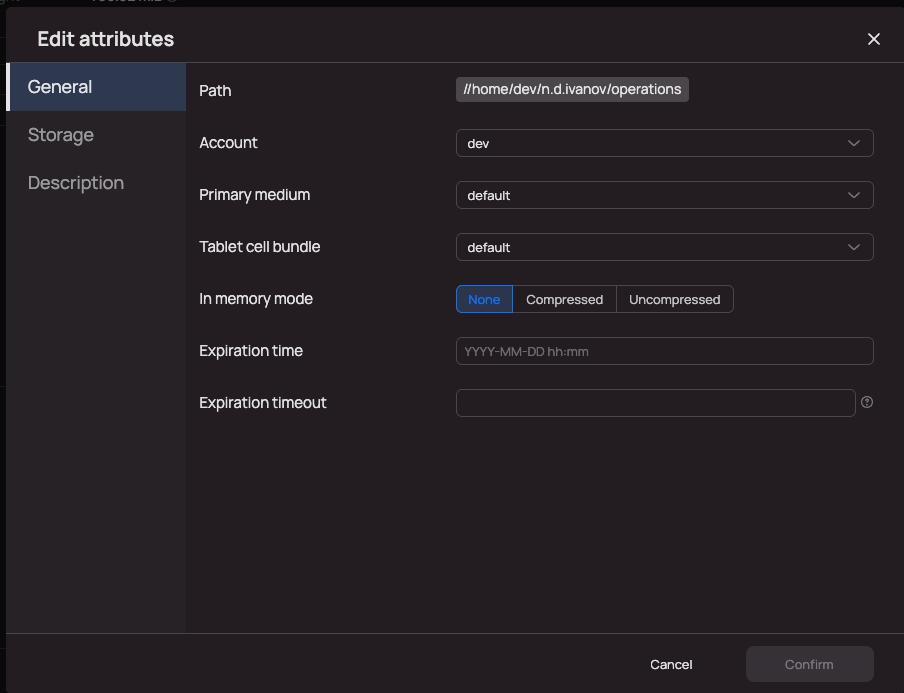
\includegraphics[width=5.15cm]{../YTsaurus/yt_1.jpg}%
  };

  \node[
    anchor=north west,
    fill=softcyan,
    rounded corners=10pt,
    text width=6.3cm,
    inner xsep=0.35cm,
    inner ysep=0.24cm,
    align=left
  ] at ([xshift=0.95cm,yshift=-1.95cm]current page.north west) {%
    {\fontsize{8.8}{10.1}\selectfont
    \textbf{Модель хранения}\\[0.10cm]
    Одна dynamic table, где каждая строка соответствует отдельной операции.\\
    Составной ключ: \texttt{objectId}, \texttt{replicaId}, \texttt{txId}, \texttt{opId}.}%
  };

  \node[
    anchor=north west,
    fill=softgray,
    rounded corners=10pt,
    text width=6.25cm,
    inner xsep=0.30cm,
    inner ysep=0.24cm,
    align=left
  ] at ([xshift=0.95cm,yshift=-4.35cm]current page.north west) {%
    {\fontsize{8.6}{9.6}\selectfont
    \textbf{Особенности}\\
    • ориентирован на большой объём и распределённое выполнение;\\
    • хорошо работает с запросами по префиксу ключа.\\[0.16cm]
    \textbf{Риск}\\
    Поиск по \texttt{action.path} требует полного чтения истории объекта\\
    с последующей фильтрацией в Java.}%
  };

\end{tikzpicture}

\footerband{6}
